\documentclass[twocolumn]{article}

\usepackage{amsmath, amssymb, amsthm}
\usepackage{tikz}
\usetikzlibrary{arrows,decorations.markings}
\usetikzlibrary{calc}
\usetikzlibrary{intersections}
\usetikzlibrary{positioning}
\usetikzlibrary{patterns}
\usetikzlibrary{circuits.logic.US,circuits.logic.IEC,fit}
\newcommand\addvmargin[1]{
  \node[fit=(current bounding box),inner ysep=#1,inner xsep=0]{};
}
\usepackage{pgfplots}
\usepgflibrary{patterns}
\usepackage[T1]{fontenc}
\usepackage{CrimsonPro}
\usepackage{multirow}
\usepackage{footnote}
\makesavenoteenv{tabular}
%\usepackage[russian]{babel}
\usepackage{CJKutf8}
\usepackage{forest}
\usepackage{textcomp}
\usepackage{multicol}
\usepackage{booktabs}
\usepackage{float}
\usepackage{makecell}
\usepackage[makeroom]{cancel}
\usepackage{lscape}
\usepackage[utf8]{inputenc}
\usepackage{geometry}
 \geometry{
 a4paper,
 left=10mm,
 right=10mm,
 top=10mm,
 bottom=20mm,
}
\usepackage{hyperref}

\newcommand{\idk}{\begin{CJK}{UTF8}{ipxm} ¯\textbackslash \_(ツ)\_/¯ \end{CJK}}
\newcommand{\thicc}{thick}
\newcommand{\ultraskip}{\bigskip\bigskip\bigskip\bigskip\bigskip\bigskip}
\newcommand{\tabellenskalierung}{0.75}
\newcommand{\PreserveBackslash}[1]{\let\temp=\\#1\let\\=\temp}
\newcolumntype{C}[1]{>{\PreserveBackslash\centering}p{#1}}
\newcolumntype{R}[1]{>{\PreserveBackslash\raggedleft}p{#1}}
\newcolumntype{L}[1]{>{\PreserveBackslash\raggedright}p{#1}}

\title{Wirtschaftsinformatik Glossar}
\author{Jonas Walkling}

\begin{document}


\section{Hardware}

Alle physischen Teile eines Computers. 

\paragraph{EVA}
	\begin{itemize}
		\item[E]ingabe
		\item[V]erarbeitung
		\item[A]usgabe
	\end{itemize}

\paragraph{Input Kategorisierung\\\\}
	\begin{forest} for tree={grow'=0,anchor=west},
		[Input [Halbdirekt [Urbeleg] [Plastikkarten]]  [Direkt [Automatisch][Manuell[Online-Datenerfassung][Dialog-Eingabe]] [Akustisch]]]
	\end{forest}

\begin{figure}[H]
	\paragraph{$\qquad \quad$ Informationssystem Eingabe\\\\}
\advance\leftskip-1.2cm
\begin{tabular}{L{30mm}L{30mm}L{30mm}}
	\toprule
	\multicolumn{3}{c}{Eingabe/Kodierung} \\
	\cmidrule(l){1-3}
	\textbf{verhalten} & \textbf{eingeben} & \textbf{bedienen(IT)} \\
	\textbf{nicht kommunizieren} & sprechen & Tastatur \\
	laufen, blicken & schreiben & Maus/Stift \\
	\textbf{kommunizieren} & zeichnen & Toucheingabe \\
	sprechen & fotografieren & \\
	sprechen, gestikulieren \\
	\cmidrule(l){1-3}
	\textbf{aufnehmen} & \textbf{erkennen} & \textbf{weiterverarbeiten} \\
	-
	Bild aufnehmen     &  Bilder interpretieren & Daten \\
	Sprache aufnehmen& Sprache erkennen \\
	Blicke registrieren& Emotionen interpretieren \\
	Handschrift erkennen& Schrift Erkennen \\
	Musik aufnehmen& Musik klassifizieren \\
	\bottomrule
\end{tabular}
\end{figure}

\paragraph{Texteingabe Beispiel}
\begin{itemize}
	\item Tastatur
	\item Digitalstift
	\item Infrarottastatur
	\item Handbewegungserkennung
	\item OCR (Optical Character Recognition)
\end{itemize}

\paragraph{Sprache}
ist für den Menschen einfacher, da sie natürlicher ist. Für Maschinen ist sie schwieriger, da die Mustererkennung deutlich schwieriger ist. 

Problemlösungen:\footnote{Ich habe mal wieder keine Ahnung, was mit dieser Liste vermittelt werden soll. Nummer 1 und 2, sind offensichtliche Voraussetzungen für einen Sprachassistenten. Was diese nebulösen MID sein sollen, bleibt wohl ein Geheimnis und das in Punkt 4 steht, dass Test zur Funktion gemacht werden hätte ja auch keiner Ahnen können \idk}
\begin{enumerate}
	\item Erhebung von relevantem Vokabular, Satzkonstruktionen
	\item Aussprachelexika
	\item Mixed-Initiative-Dialoge: Sammlung möglicher Antworten
	\item Tests und Trainings in Sprachlaboren
\end{enumerate}

\paragraph{Bilder} sind modernerer Technik auswertbar zum Beispiel kann erkannt werden, was auf einem Bild zu sehen ist.
\begin{itemize}
	\item algorithmisch: Algorithmen zur Bildzerlegung und -interpretation \footnote{Das algorithmische Verarbeitung Algorithmen erfordert ist ja fast schon ein Pleonasmus}
	\item Lernende Verfahren: \footnote{Natürlich sind Lernende Verfahren keine Algorithmen (Das war Sarkasmus)} Neuronale Netze üben menschliches Erkennen \footnote{Dem Verfasser dieses Satzes war entweder nicht bewusst wie Menschen funktionieren oder wie neuronale Netze funktionieren. Ich vermute stark das beides der Fall war.}
\end{itemize}

\paragraph{Smartphone Sensoren}
\begin{itemize}
	\item Mikrofon
	\item Kamera
	\item Berührung
	\item GPS/ГЛОНАСС/Gallileo
	\item Magentfeld
	\item Rotation
	\item Näherung
	\item Helligkeit
	\item Thermometer
	\item Voltmeter
	\item Fingerabdruck
\end{itemize}

\paragraph{Zentraleinheit \\\\}
	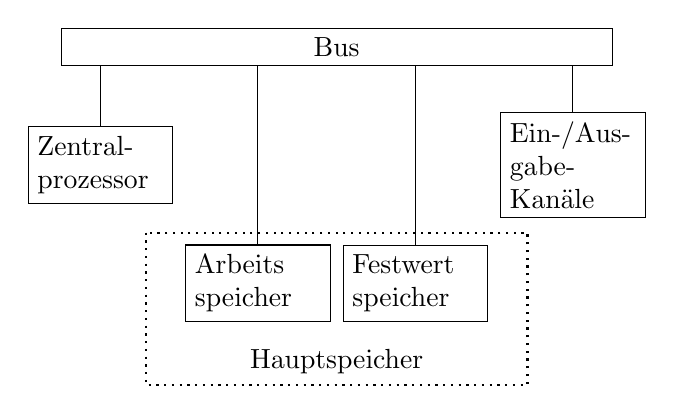
\begin{tikzpicture}
		\path 	(2,3)	node[draw, minimum width=70mm] (a) 	{Bus}
			(-1,1.5)	node[draw, text width=16mm] (b)  	{Zentral\-prozessor}
			(5,1.5)	node[draw, text width=16mm] (c)  	{Ein-/Aus\-gabe\-Kanäle}
			(1,0)	node[draw, text width=16mm] (d)  	{Arbeits speicher}
			(3,0)	node[draw, text width=16mm] (e)  	{Festwert speicher};
		\draw (b) to (b|-a.south);
		\draw (c) to (c|-a.south);
		\draw (d) to (d|-a.south);
		\draw (e) to (e|-a.south);
 			\draw[thick,dotted]     ($(d.north west)+(-0.5,0.15)$) rectangle ($(e.south east)+(0.5,-0.8)$);
		\draw (2,-1) node {Hauptspeicher};
	\end{tikzpicture}

\paragraph{Zentralprozessor \\\\}
	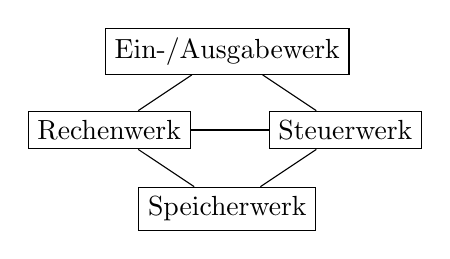
\begin{tikzpicture}
		\path 	(2,2)	node[draw] (a) 		{Ein-/Ausgabewerk}
			(0.5,1)	node[draw] (b)  	{Rechenwerk}
			(3.5,1)	node[draw] (c)  	{Steuerwerk}
			(2,0)	node[draw] (d)  	{Speicherwerk};
		\draw (a) to (b) to (d) to (c) to (a);
		\draw (b) to (c);
	\end{tikzpicture}

\paragraph{Qualitätsmerkmale des Zentralprozessors}
	\begin{itemize}
		\item Zykluszeit bzw. Taktfrequenz
		\item Verarbeitungsbreite (z.B. 64-Bit)
		\item Instruktionsrate (Instruktionen pro Sekunde) \footnote{An dieser Stelle werden im Skript die Akronyme MIPS und MFLOPS genannt. Dies ist insofern irreführend als das sich "million instructions per second" (MIPS) auf die Anweisung die der Prozessor ausführt bezieht, während "million floating point operations per second" (MFLOPS) auf die Geschwindigkeit bei der Multiplikation großer Zahlen bezieht. MFLOPS sind in der Regele ein besseres Maß für die Performance einer CPU. Allerdings sind sie anders als im Skript dargestellt kein Maß für die Instruktionsrate.}
		\item Befehlsvorrat (Cache)
		\item Architektur (z.B. x86, ARM)
	\end{itemize}

\paragraph{Rechnerarchitekturen \\	}
	\begin{forest} [[Rechnerarchitekturen [von-Neumann\\-Architektur, align=center] [Parallele \\Architektur ,align=center [Pipeline-System] [Multiprozessorsysteme [Asymmetrische Systeme] [Symmetrische Systeme]]]]]
	\end{forest}

\paragraph{Flüchtiger Speicher}
	Speicher die nur mit konstanter Stromversorgung Informationen speichern können (RAM, SRAM, VRAM)

\paragraph{(D)RAM}
	(Dynamic) Random Access Memory / Arbeitsspeicher \\
	Besteht aus Speicherzellen die wiederum aus einem Transistor und Kondensator. Dieser muss mehrere tausend mal pro Sekunde neu beschrieben werden um die Entladung der Kondensatoren zu verhindern.

\paragraph{SRAM}
	Static Random Access Memory / CPU-Cache \\
	Muss im gegensatz zu DRAM \textit{NICHT} neu beschrieben werden und besteht aus komplexeren Speicherzellen (Boolean-Gate). Dadurch ist er teurer aber schneller als DRAM.

\paragraph{Nicht-flüchtige Direktzugriffsspeicher}
	Speicher bei denen an jeder beliebigen Stelle mit dem Lesen begonnen werden kann (USB, CD, HDD, SSD)

\paragraph{Nicht-flüchtige sequentielle Speicher}
	Speicher bei denen beim Lesevorgang alle Daten zwischen der aktuellen und gewünschten Position gelesen werden müssen (Kassette)

\paragraph{3-Schichten-Modell}
\begin{itemize}
	\item Hardware
	\item Software 
	\item Betriebssystem
\end{itemize}

\section{Software}

	\begin{flushleft}
	\begin{forest}
	[Software \footnotemark,draw 			
	[Systemsoftware,draw 
		[Betriebssystem
		[Übersetzungsprogramm \footnotemark
		[Dienstprogramme \footnotemark
		[Protokolle\footnotemark und Treiber\footnotemark ]]]]]
	[Anwendungs\\software,draw, align=center
		[Standardsoftware 
		[Basissoftware 
		[Bürosoftware 
		[betriebliche Software ]]]] 
		[Individual\\software, align=center]]]
	\end{forest}
	\end{flushleft}
\footnotetext[2]{Hier möchte ich anmerken, dass diese Grafik -- zumindest bei alleiniger Konsultation des Skriptes -- keiner mir erkennbaren Logik folgt und nur aus vollkommen willkürlich zusammengewürfelten Wörtern besteht. Verständlich wird es erst mit der Zuhilfenahme des Buches "Grundzüge der Wirtschaftsinformatik" von Peter Mertens Die Obigen Erklärungen sind diesem entnommen. Dem Skript scheint es zu mühselig zu sein verwendete Begriffe zu erklären.}
\footnotetext[3]{Compiler / Interpreter}
\footnotetext[4]{Dies sind Programme welche allgemeine Aufgaben erledigen, wie das Kopieren von Dateien oder die Verbindung zu einem WLAN-Netz}
\footnotetext[5]{Mir ist nicht ganz klar, warum hier Protokolle erwähnt werden bzw. welche Protokolle gemeint sind. Die meisten Netzwerkprotokolle wie HTTP, FTP, oder SMTP (e-mail) werden von den sie nutzenden Anwendungen selber implementiert. Auch eine  SSH Implementierung bei UNIX-Systemen würde ich eher als Dienstprogramm kategorisieren.}
\footnotetext[6]{Bei Windows nicht. lol}

\paragraph{Customizing}
	Die Anpassung von Standardsoftware an spezielle Bedürfnisse von Nutzern.


\paragraph{Fakturierung \\}
	Rechnungsstellung

\paragraph{Software}
	\texttt{Definition aus der Vorlesung:} \\ 
	PrOgRaMmE, dIe iN eInEr PrOgRaMmIeRsPrAcHe gEscHriEbEn sInD. \\
	\texttt{Sinnvolle Definition:} \\
	Eine Ansammlung von Daten oder Instruktionen, die in einem Computersystem ein bestimmtest Verhalten hervorruft. \\\\


\paragraph{Informationssystem}
	Informationssysteme sind soziotechnische Systeme aus Mensch und Technik zur Erfüllung einer Aufgabe. Sie erfassen, verarbeiten, speichern und übertragen Informationen.

\paragraph{Anwendungssysteme} Anwendungssysteme sind technische Systeme aus Hard- und Software (im 
Informationssystem). 

\paragraph{Gestaltung von informationssystemen im Unternehmen}
\begin{itemize}
	\item Konzeption
	\item Entwicklung
	\item Einführung
	\item Wartung
	\item Nutzung
	\item Zielgerichteter Einsatz
\end{itemize}

\paragraph{Gestaltung von Informationssystemen in der Wirtschaft \\}
	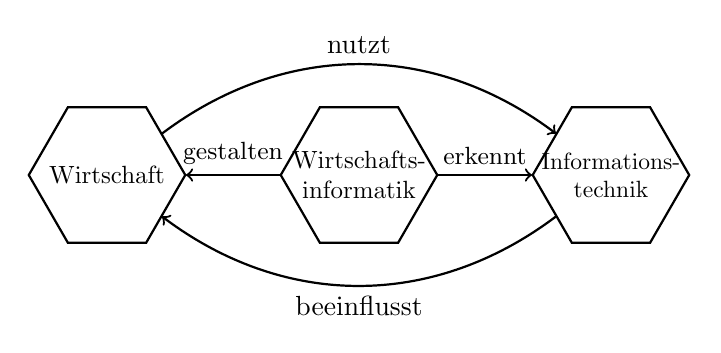
\begin{tikzpicture}
		[thick]
		\coordinate (a) at (0,0);
		\coordinate (b) at (3.2,0);
		\coordinate (c) at (6.4,0);
		\draw (a) node[text centered, text width=20mm, scale=0.9] (d) {Wirtschaft};
		\draw (b) node[text centered, text width=20mm, scale=0.9] (e) {Wirtschafts\-informatik};
		\draw (c) node[text centered, text width=22mm, scale=0.85] (f) {Informations\-technik};
		\draw (a) node[draw, regular polygon, regular polygon sides=6, text centered, text width=22mm, scale=0.5] (d) {};
		\draw (b) node[draw, regular polygon, regular polygon sides=6, text centered, text width=22mm, scale=0.5] (e) {};
		\draw (c) node[draw, regular polygon, regular polygon sides=6, text centered, text width=22mm, scale=0.5] (f) {};
		\draw[<-] (d) to node[midway, above] {\small gestalten} (e);
		\draw[->] (e) to node[midway, above] {\small erkennt} (f);
		\draw[->] (d) edge [bend left=37] node[midway, above] {nutzt} (f);
		\draw[<-] (d) edge [bend right=37] node[midway, below] {beeinflusst} (f);
	\end{tikzpicture}
\paragraph{Cloud-Computing Merkmale}
	\begin{itemize}
		\item On-Demand Self-Service
		\item Ubiquitärer Netzwerkzugriff
		\item Standortunabhängiges Ressourcen-Pooling
		\item Elastische Kapazitäten
		\item Messbarer Dienst
	\end{itemize}

\paragraph{Cloud-Computing Arten}
	\begin{itemize}
		\item Application-as-a-Service AaaS
		\item Platform-as-a-Service PaaS
		\item Infrastructure-as-a-Service IaaS
		\item Software-as-a-Service SaaS
	\end{itemize}

\paragraph{Big Data}
Eigenschaften:
\begin{itemize}
	\item Volumen - Menge
	\item Variety - Geschwindigkeit, der Generierung
	\item Velocity - Vielfalt
	\item Value - Wert
	\item Veracity - Wahrhaftigkeit
\end{itemize}
Analysemthoden:
\begin{itemize}
	\item Business Intelligence
	\item Busniess Analytics
	\item Machine Learning
	\item Beal Time Analytics 
	\item Bildanalyse
\end{itemize}

\paragraph{Boolian-Logic}
	Kann mit den Wahrheitswerten 0 und 1 arbeiten.

\paragraph{Fuzzy-Logic}
	Kann mit Wahrheitswerten zwischen 0 und 1 arbeiten.

\paragraph{Neuronale Netze}
Ein Wage an das menschliche Gehirn angelehntes Netz von Input, Hidden und Outputnodes. Im Prinzip handelt es sich um eine n-Dimensionale Funktion die das Maximum bzw. Minimum errechnet. Das System kann mit Daten trainiert werde, wobei bestimmte Parameter im System angepasst werden. Ein Neuron wird aktiviert wenn wenn die gewählte Funktion multipliziert mit der gewichteten Summe der Inputs großer ist als der Wert des Node. Diese Operationen wird dann für alle Nodes des Neuronalen Netzes von links nach rechts ausgeführt. In der Praxis wird dies mit Matrixmultiplikationen durchgeführt, welche in den meisten Programmiersprachen stark optimiert und dadurch sehr effizient ist.
\begin{equation*}
f \left(\text{Bias} + \sum_{i=1}^{n} \text{Input}_i \cdot \text{Weight}_i \right) > \text{Node}
	\end{equation*}
	
	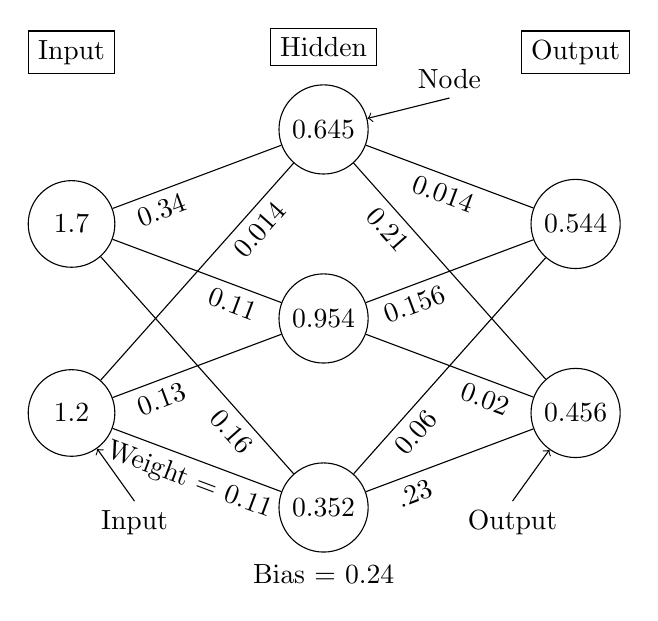
\begin{tikzpicture}
		[scale = 1.6]
		\coordinate (a) at (0,0);
		\coordinate (b) at (0,1.5);
		\coordinate (c) at (2,-0.75);
		\coordinate (d) at (2,0.75);
		\coordinate (e) at (2,2.25);
		\coordinate (f) at (4,0);
		\coordinate (g) at (4,1.5);

		\path
		(a) node[draw,circle, minimum size=1.1cm](o) {1.2}
		(b) node[draw,circle, minimum size=1.1cm](p) {1.7}
		(c) node[draw,circle](q) {0.352}
		(d) node[draw,circle](r) {0.954}
		(e) node[draw,circle](s) {0.645}
		(f) node[draw,circle](t) {0.456}
		(g) node[draw,circle](u) {0.544};
		
		\draw (q) node[below=0.6cm] {Bias = 0.24};
		\draw[->] (0.5,-0.7) node[below] {Input} to (o);
		\draw[->] (3.5,-0.7) node[below] {Output} to (t);
		\draw[->] (3,2.5) node[above] {Node} to (s);

		\draw (b) node[above=19mm,draw] {Input};
		\draw (e) node[above=8mm,draw] {Hidden};
		\draw (g) node[above=19mm,draw] {Output};
		\draw (o) to node[below, sloped, midway] {Weight  = 0.11} (q) to node[below, sloped, near start] {.23} (t) to node[below, sloped, near start] {0.02} (r) to node[below, sloped, near end] {0.13} (o);
		\draw (p) to node[below, sloped, near start] {0.34} (s) to node[below, sloped, midway] {0.014} (u) to node[below, sloped, near end] {0.156} (r) to node[below, sloped, near start] {0.11} (p);
		\draw (o) to node[below, sloped, near end] {0.014} (s) to node[below, sloped, near start] {0.21} (t);
		\draw (p) to node[below, sloped, near end] {0.16} (q) to node[below, sloped, near start] {0.06} (u); 
	\end{tikzpicture}

\paragraph{EDI}
	Electronic Data Interchange

\paragraph{CAQ}
	Computer-aided quality

\paragraph{CAM}
	Computer aided manufacturing

\paragraph{CAD}
	Computer aided design

\paragraph{CAE}
	Computer aided engineering

\paragraph{CAP}
	Computer aided planning

\paragraph{PPS}
	Production planning System

\paragraph{ERP}
	Enterprise resource planning

\paragraph{WGSS}
	 Workgroup-Support-Systeme \\
	 unterstützt Themas bei der Bearbeitung eher unstrukturierter Aufgaben, wobei die Teamarbeit meist orts- und zeitunabhängig erfolgt.

\paragraph{RFID}
	Radio-frequency identification

\paragraph{NFC}
	Near-field communication
\paragraph{Prozessorientierung}
	Hierbei wird der Fokus der Betrachtung auf einen Prozess gelegt. Zum Beispiel die Konzeptionierung und Auslieferung eines Produktes vom Beginn bis zum Ende. 

\paragraph{Funktionsorientierung}
	Hierbei wird der Fokus der Betrachtung auf eine Funktionseinheit gelegt. Zum Beispiel den Vertrieb einer Firma.

\paragraph{Client-Server}
	Ein Nutzer (Client) greift auf Services oder Daten auf einem zentralen Computer (Server) zu. 
	\begin{itemize}
		\item File-Server \\  Datenspeicher
		\item Multimedia-Server \\ Datenspeicher
		\item Datenbank-Server \\ Datenspeicher (für mehr Daten) 
		\item Kommunikations-Server \\ Regelt die Kommunikation zwischen Netzwerken
		\item Mail-Server \\ Versenden von Daten zwischen Nutzern. Meist nach dem SMTP (senden) und IMAP/POP3 (empfangen) Protokoll     
	\end{itemize}

\paragraph{P2P}
	System zur Datenübertragung, bei dem Daten direkt zwischen den Teilnehmern hin und her gesendet werde. Dabei wird kein Zentraler Server benötigt.
	\begin{itemize}
		\item File-Sharing \\
			Dateienaustausch zwischen Teilnehmern.
		\item Ressource-Sharing \\
			Das Verteilen von Rechenoperationen auf die teilnehmenden Peers (Nutzer)
		\item Collaboration \\
			Verteilte Zusammenarbeit (Im Prinzip die beiden davor kombiniert)
	\end{itemize}

\paragraph{Netzkonzepte\\}
	\begin{tabular}{L{25mm}|L{25mm}|L{25mm}}
		Mainframe \footnotemark  & Peer-to-Peer & Client-Server \\ \hline
		 zentrale Rechenanlage & gleichartige Rechner & Server Stellt Dienste zur Verfügung \\ \hline
		  einfache Verwaltung & schnell einzurichten / billig  & Günstiger als Mainframe \\ \hline
		  Ausfall des Mainframe bedeutet Ausfall des gesamten Netzes & aufwendige Verwaltung & Serverausfall bedeutet Dienstausfall  \\
	\end{tabular}

\footnotetext[1]{Exkurs zum Thema Mainframe: Ein Mainframe ist eigentlich ein für Firmenanwendungen ausgelegter Computer, der sich vor allem durch seine Zuverlässigkeit und hohe Datenverarbeitungsrate auszeichnet. Die Zuverlässigkeit wird vor allem durch die Redundanz von Teilen erreicht. So sind Speicher oder Netzwerkcontroller mehrmals vorhanden. So bleibt die Funktion beim Ausfall von einzelnen Teilen gewährleistet. Dies ist häufig auch durch "Hot-swapping" möglich. Das bedeutet, dass Hardware im laufenden Betrieb gewechselt werden kann. Die hohe Datenverarbeitung wird durch eine hohe Anzahl an I/O (Input/Output) erreicht. Oft haben Mainframes Subprozessoren die nur dafür Verantwortlich sind die ein und ausgehenden Datenströme zu erfassen und weiterzuleiten. Zusätzlich sind Mainframes auf Langlebigkeit der Software ausgelegt, so dass Anwendungen über Jahre oder Jahrzehnte betrieben werden können. Die Serverausfallzeiten des IBM Z -- dem vermutlich verbreitetsten Mainframe -- lagen im Jahre 2018 im Schnitt bei ca. 0.94 Sekunden pro Jahr. TLDR: Das was im Skript steht hat nichts damit zu tun, was einen Mainframe-Computer ausmacht.}

\paragraph{DSDL}
	Data Storage Description Language \\
	Eine Speicherbeschreibungssprache zur Beschreibung der physischen Datenorganisation, die keiner mehr braucht, seit es SQL gibt.

\paragraph{DBMS}
	Datenbankmanagementsystem \\
	System zur Verwaltung von Datenbanken. Das DBMS dient auch der Abfrage von Daten und als Interface für den Nutzer.

\paragraph{DB}
	Datenbank \\
	Persistenter Speicherort für die Daten eines Datenbanksystems.

\paragraph{Datenbanksystem}
	DBMS + DB

\paragraph{Dialogverarbeitung}
	Computersystem, dass die Aufträge verschiedener Nutzer an einem System nacheinander abarbeitet (Batch/Stapelverarbeitung) und nach Beendigung eines Arbeitsauftrages den Output an den Nutzer zurück gibt.

\paragraph{MRP I \\}
	Material Requirements Planning / Materialbedarfsplanung 
	\begin{itemize}
		\item Zu produzierende Teile
		\item Zu beschaffende Teile
		\item Direkte Materialien
		\item Indirekte Materialien
	\end{itemize}

\paragraph{MRP II}
	Manufacturing Ressource Planning 

\paragraph{MPS}
	Master Production Schedule

\paragraph{ROM}
	read-only-memory / Festwertspeicher


\paragraph{Web Service}
	\begin{itemize}
		\item modular
		\item plattformunabhängig
		\item implementierungsunabhängig
		\item Anwendung oder Dienst
	\end{itemize}

\paragraph{E-Commerce}
	Elektronischer Vertrieb von Produkten \\\\
	\begin{tabular}{L{19mm}|L{30mm}|L{27mm}}
		\multicolumn{3}{c}{Basismodell des E-Commerce} \\ \hline
		Transaktions\-phasen & 
		Aufgaben und Prozesse & 
		Apps Websites  \\ \hline
		Anbahnung&Informationssuche Klärung vorvertraglicher Probleme  & Präsentations-, Auskunfts-, Beratungssysteme  \\ \hline
		Vereinbarung&Leistungsspezifikation, Preisverhandlung, Vertragsabschluss  & Konfigurationssystem Preisfindungssystem (Auktion) \\ \hline
		Durchführung & Überwachung des Leistungsaustauschs Auswahl Zahlungsmittel & Trackung und Tracing Systeme \\
	\end{tabular}

\paragraph{Anforderungen an Software}
	\begin{itemize}
		\item Funktionsfähigkeit
		\item Usability
		\item Design
	\end{itemize}

\paragraph{Wert \protect\footnote{Die Definition des Begriffes Wert, welcher im Skript inflationär gebraucht, jedoch nie definiert wird, ist laut dem Duden "einer Sache innewohnende Qualität, aufgrund deren sie in einem gewissen Maße begehrenswert ist [und sich verkaufen, vermarkten lässt]". Demzufolge ist es eigentlich für eine Beschreibung und Klassifikation von Qualitäten völlig ungeeignet, da es keinerlei Aussage über tatsächliche Eigenschaften trifft. Das Wort reiht sich also wunderbar in den Rest der Vorlesung, als Platzhalter ohne echten Inhalt, fabelhaft ein.}
von Software}
	\begin{itemize}
		\item für den Nutzer
		\item für seine Prozesse under Erwartungen
		\item als Service
		\item Zufriedenheit
	\end{itemize}

\paragraph{Funktion Sozialer Medien}
	\begin{itemize}
		\item Vernetzen
		\item Wissen
		\item Soziale Nähe
	\end{itemize}

\paragraph{Mensch vs IT \\}
\begin{tabular}{llllll}
	Wahrnehmung & Sensoren \\
	Intelligenz & KI \\
	Gedächtnis & Big Data \\
	Reaktion & Effektoren \footnotemark
\end{tabular}
\footnotetext[5]{Apps, Bots, Agenten (Was auch immer letzteres soll \idk }

\paragraph{Digitale Transformation\\} 

\paragraph{Informationssysteme} sind soziotechnische Systeme aus Mensch und Technik zur Erfüllung einer Aufgabe sie erfasse, verarbeiten, speichern und übertragen Informationen.

\paragraph{Anwendungssysteme} sind technische Systeme aus Hard- und Software (im Informationssystem)


\paragraph{Wissen}
	Gesamtheit der Kenntnisse und Fähigkeiten eines Individuums.

\paragraph{Ideenmanagement}
	Steuerung und Förderung von Kreativität in Organisationen.

\paragraph{Innovationsmanagement}
	Systematische Planung, Steuerung und Kontrolle der Innovation in der Organisation. Beschäftigt sich jedoch im gegensatz zum Ideenmanagemnt nicht mit Kreativität sonder mit ihrer Verwertung.

\paragraph{Wissensmanagement}
	Methodische Einflussnahme auf die Wissensbasis der Organisationen.

\paragraph{Wissensbasis}
	Das angesammelte und dokumentierte Wissen.

\paragraph{Übergang Zeichen $\rightarrow$ Wissen \\}
	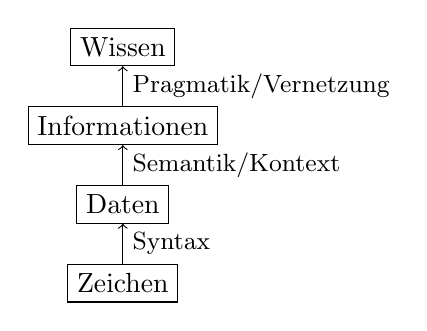
\begin{tikzpicture}
		\path
		(5,4) node[draw](a) {Wissen}
		(5,3) node[draw](b) {Informationen}
		(5,2) node[draw](c) {Daten}
		(5,1) node[draw](d) {Zeichen};
		\draw[<-] (a) to node[right] {\small Pragmatik/Vernetzung} (b);
		\draw[<-] (b) to node[right] {\small Semantik/Kontext} (c);
		\draw[<-] (c) to node[right] {\small Syntax} (d);
	\end{tikzpicture}

\paragraph{Implizites Wissen}
	Schwer zu formulierendes oder weiterzugebendes Wissen. Nicht für alle zugänglich. Erfahrungswissen.

\paragraph{Explizites Wissen}
	Systematisiertes und allgemein zugängliches Wissen, für das mediale Aufzeichnungen Existieren.

\paragraph{Externalisierung}
	Die Umwandlung von implizitem zu explizitem Wissen.

\paragraph{Information Stickiness}
	Wissen klebt \footnote{Ja! Das steht so im Skript.}
	Informationen lassen sich nur schwer Weitergeben.

\paragraph{Wissenstreppe nach North\\}
	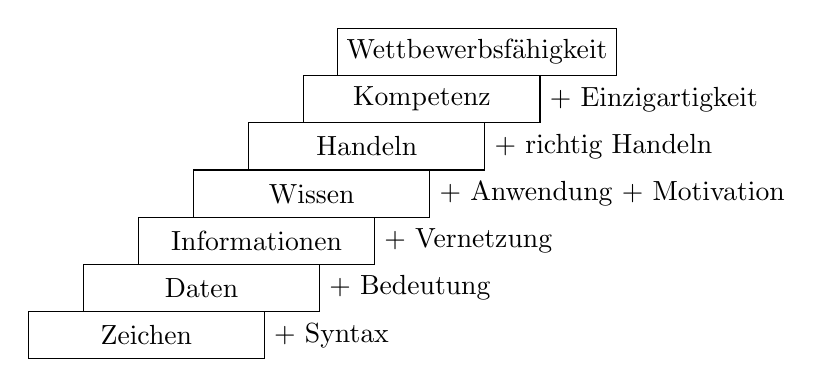
\begin{tikzpicture}
		\path
		(0.0,0.0) node[draw, minimum height=6mm, minimum width=30mm] (a) {Zeichen}
		(0.7,0.6) node[draw, minimum height=6mm, minimum width=30mm] (b) {Daten}
		(1.4,1.2) node[draw, minimum height=6mm, minimum width=30mm] (c) {Informationen}
		(2.1,1.8) node[draw, minimum height=6mm, minimum width=30mm] (d) {Wissen}
		(2.8,2.4) node[draw, minimum height=6mm, minimum width=30mm] (e) {Handeln}
		(3.5,3.0) node[draw, minimum height=6mm, minimum width=30mm] (f) {Kompetenz}
		(4.2,3.6) node[draw, minimum height=6mm, minimum width=30mm] (g) {Wettbewerbsfähigkeit};

		\draw (a) node[right=15mm] {+ Syntax};
		\draw (b) node[right=15mm] {+ Bedeutung};
		\draw (c) node[right=15mm] {+ Vernetzung};
		\draw (d) node[right=15mm] {+ Anwendung + Motivation};
		\draw (e) node[right=15mm] {+ richtig Handeln};
		\draw (f) node[right=15mm] {+ Einzigartigkeit};
	\end{tikzpicture}


\paragraph{Industrie 1.0}
	Automatisierung durch Dampfkraft, Mechanisierung

\paragraph{Industrie 2.0}
	Fließbandarbeit, Elektrifizierung, Massenproduktion

\paragraph{Industrie 3.0}
	Automatisierung, Computer

\paragraph{Industrie 4.0}
	Cyber-physische Systeme, Netzwerke, Internet der Dinge

\paragraph{ Yield-Management / Ertragsmanagement}
	Ein, meist rechnergestütztes Preissteuerungssystem, bei dem es nicht nur Preisdifferenzierung zwischen den Produkten sondern auch innerhalb eines Produktes gibt. Ein beispiel wäre die Preisgestaltung von Flugtickets, die abhängig von der Zeit der Bestellung im Preis variieren. Hierzu werden statistische Prognoseverfahren eingesetzt um das Verhalten der Käufer vorauszusehen.

\paragraph{Wirtschaftliche Transaktion \\}
	\begin{tabular}{L{20mm}|L{30mm}|L{30mm}}
		\begin{tabular}{l} Transaktions- \\ phasen \end{tabular} & Aufgaben & IT-System \\ \hline
		Anbahnung&Informationssuche Klärung vorvertraglicher Probleme  & Präsentations-, Auskunfts-, Beratungssysteme  \\ \hline
		Vereinbarung&Leistungsspezifikation, Preisverhandlung, Vertragsabschluss  & Konfigurationssystem Preisfindungssystem (Auktion) \\ \hline
		Durchführung & Überwachung des Leistungsaustauschs Auswahl Zahlungsmittel & Trackung und Tracing Systeme \\
	\end{tabular}

\paragraph{Geschäftsprozess}
	\begin{itemize}
		\item verarbeitet \textbf{Informationen} 
		\item hat einen definierten \textbf{Beginn}  und ein definiertes \textbf {Ende}
		\item besteht aus mindestens zwei \textbf{Aktivitäten}
		\item erzeugt ein eindeutiges, abgrenzbares \textbf{Ergebnis}
	\end{itemize}

\paragraph{BPO}
	Business Process Outsourcing \\
	Die Auslagerung von ganzen Geschäftsprozess inklusive ihrer IT-Systeme.

\paragraph{EPK} Ereignissgesteuerteprozesskette \\

\end{document}

